\documentclass[twoside]{article}

%-------------------------------------------------------------------------------

\usepackage{amsthm}
\usepackage[sc]{mathpazo} 	% palatino font
\usepackage[T1]{fontenc} 	% 8-bit encoding; 256 glyphs
\linespread{1.05} 			% line spacing
\usepackage{microtype} 		% slightly tweak font spacing
\PassOptionsToPackage{usenames,dvipsnames,svgnames}{xcolor}  
\usepackage{tikz}
\usetikzlibrary{arrows,positioning,automata}
\usepackage[hmarginratio=1:1,top=32mm,columnsep=20pt]{geometry} 	% Document margins
\usepackage{multicol} 												% two-column layout
\usepackage[hang, small,labelfont=bf,up,textfont=it,up]{caption} 	% float captions
\usepackage{booktabs} 		% Horizontal rules in tables
\usepackage{float} 			% allows tables/figures in the multi-column environment
\usepackage{hyperref} 		% hyperlinks in the PDF
\usepackage{subfig}			% figures inside of figure environment
\usepackage{lettrine} 		% large first letter
\usepackage{paralist} 		% compactitem environment
\usepackage{abstract} 		% abstract customization
\renewcommand{\abstractnamefont}{\normalfont\bfseries} 		% bold abstract text
\renewcommand{\abstracttextfont}{\normalfont\small\itshape} % small italic abstract

\newtheorem{theorem}{Theorem}

\usepackage{titlesec} 							% title customization
\renewcommand\thesection{\Roman{section}} 		% roman numerals for the sections
\renewcommand\thesubsection{\Roman{subsection}} % roman numerals for subsections
\titleformat{\section}[block]{\large\scshape\centering}{\thesection.}{1em}{} % Change the look of the section titles
\titleformat{\subsection}[block]{\large}{\thesubsection.}{1em}{} % Change the look of the section titles

\usepackage{algorithm}
\usepackage{algorithmicx}
\usepackage[noend]{algpseudocode}
\usepackage{fontspec}
\newcommand*\Let[2]{\State #1 $\gets$ #2}

\algrenewcommand\algorithmicrequire{\textbf{Precondition:}}
\algrenewcommand\algorithmicensure{\textbf{Postcondition:}}

\usepackage{fancyhdr} 	% Headers and footers
\pagestyle{fancy} 		% All pages have headers and footers
\fancyhead{} 			% Blank out the default header
\fancyfoot{} 			% Blank out the default footer
\fancyhead[C]{Algorithms for the Online Time Dependant Freeze-Tag Problem $\bullet$ July 2015 $\bullet$ Dan Hill} % Custom header text
\fancyfoot[RO,LE]{\thepage} % Custom footer text			% includes and document setup

%-------------------------------------------------------------------------------

\newcommand{\articletitle}{Analsysis of the Nearest Neighbor\\ Heuristic for the Online Time\\ \vspace{1.4mm} Dependant Freeze-Tag Problem}
\newcommand{\name}{Dan Hill}
\newcommand{\university}{Cameron University}
\newcommand{\email}{mail@danhill.us}


\title{\vspace{-15mm}\fontsize{24pt}{10pt}\selectfont\textbf{\articletitle}} % Article title

\author{\large\textsc{\name} \\[2mm] 		% Your name
\normalsize \university \\		 			% Your institution
\normalsize \href{mailto:\email}{\email} 	% Your email address
\vspace{-5mm}}

\date{}			% title formatting

%-------------------------------------------------------------------------------

\begin{document}

\maketitle 				% Insert title
\thispagestyle{fancy} 	% All pages have headers and footers
%----------------------------------------------------------------------------------------
%	ABSTRACT
%----------------------------------------------------------------------------------------

\begin{abstract}

The abstract lives here.

\end{abstract}		% abstract

%-------------------------------------------------------------------------------
%	ARTICLE CONTENTS
%-------------------------------------------------------------------------------

\begin{multicols}{2} 	% Two-column layout throughout the main article text


%-------------------------------------------------------------------------------
% Introduction
%-------------------------------------------------------------------------------
\section{Introduction}
The Freeze-Tag Problem (FTP) \cite{FTP.0} is a problem in the field of swarm robotics in which a strategy to awaken a swarm in the minimum makespan must be found. In the original problem as proposed in \cite{FTP.0}, robots have two states, sleeping and awake. Sleeping robots are awakened when touched by an awake robot. 

At the beginning of the problem we are given a set of sleeping robots and a single awake robot known as the \textit{source robot}. The source robot then awakens sleeping robots which then help awaken the other robots. 

The Online Time Dependant Freeze-Tag Problem (OTDFTP) is a variation of FTP in which each robot has a release time associated with it. The OTDFTP was first proposed by Hammar et al in \cite{FTP.1}. In the OTDFTP robots have an additional state we will refer to as \textit{hibernation mode}. When A robot is in hibernation mode, it is not visible to other robots. Once a hibernating robot's release time has been reached, it will enter sleep mode and become visible to awake robots. 

\paragraph{Related Work.}
Hammer et al. \cite{FTP.1} found the Offline Time Dependant Freeze Tag Problem has a lower bound of $7/3 - \epsilon$, for any $\epsilon > 0$. 

In \cite{FTP.2}, Sztainberg et al. have proven a lower bound for the FTP using the nearest neighbor heuristic in which robots do not claim targets is at least $4-\epsilon$ times optimal for any $\epsilon > 0$\cite[Theorem ]{FTP.2}. The authors go on to find the strategy also has a tight approximation bound of $\Theta(\sqrt{\log n})$ for points on a plane and $\Theta((\log n)^{1-\frac{1}{d}})$ for points in $d$ dimensions.

\paragraph{Preliminaries.}
Let $R = \{r_0, r_1, r_2, \dots , r_n \} \subset M$ be the set of $n$ robots in some continuous metric space $M$. $M$ is a $d$-dimensional Euclidean space with distances measured according to an $L_p$ metric.Unless otherwise stated, the robot $r_0$ is the \textit{source robot} and is the only awake robot at the beginning of the problem. 

Robots have three modes: \textit{awake mode}, \textit{sleep mode}, and \textit{hibernation mode}. In awake mode, a robot is fully functional and is free to move. In hibernation mode a robot is completely inactive and can not move nor be awakened by any external means. In sleep mode, a robot is inactive but can be awakened by other awake robots by being touched.

Robots have a \textit{release time}. Once a robot's release time has passed, it will exit hibernation mode and enter sleep mode. This would be comparable to the real world example of a robot charging it's batteries and only becoming available to awaken once it's battery is full.

In order to avoid robots from traveling in a single pack, awake robots can claim a target and no other robot will target a claimed robot. \cite{FTP.2}

A solution to the OTDFTP is considered \textit{rational} if:
\begin{enumerate}
	\item Each robot with no target will immediately choose an unclaimed robot in wait mode and begin moving toward it.
	\item A robot does not move other than to advance on it's target. If a robot has no target, it will not move.
\end{enumerate}
This definition is similar to the one given in \cite{FTP.0} with slight modification for release times.
\paragraph{Summary of Results.}
We find that the competitive ratio of the Nearest Neighbor heuristic is $5/2$.

%-------------------------------------------------------------------------------
% Nearest Neighbor Algorithm
%-------------------------------------------------------------------------------
\section{The Algorithm}
The Nearest Neighbor Algorithm is a \textit{rational} wake-up strategy for the OTDFTP. Each robot chooses the closest unclaimed robot in wait mode. Once a robot has chosen a target it will not choose another target until it has reached it's current target. 
\begin{algorithm}[H]
  \caption{Returns the nearest unclaimed sleeping robot.}
  \begin{algorithmic}
    \Require{$A$ is the set of sleeping robots and $t$ be the robot's current target.}
    \Statex
    \Function{Nearest Neighbor}{$A$, $t$}
		\If{$t \neq$ NULL}
	        \State \Return $t$
        \EndIf{}
        
        \If{$A.size = 0$}
	        \State \Return NULL
	    \EndIf
	    
        \Let{$m$}{NULL}
        
        \For{$robot$ in $A$}
	        \If{$\neg robot.claimed$}
	        
				\If{$m =$ NULL}
					\Let{$m$}{$robot$}
				\Else
					\Let{$a$}{dist($self$, $robot$)}
			        \Let{$b$}{dist($self$, $m$)}
			        \If{$a < b$}
				        \Let{$m$}{$robot$}
			        \EndIf
			    \EndIf
			\EndIf
        \EndFor
        \State \Return $m$
    \EndFunction
  \end{algorithmic}
\end{algorithm}
\section{Analysis}
\begin{theorem}
For any $\epsilon > 0$, there exists an instance of the OTDFTP for which the Nearest Neighbor Algorithm results in a makespan less than $\frac{5}{2} - \epsilon$ times optimal.
\end{theorem}
\begin{proof}

\begin{figure}[H]
\tikzset{location/.style={circle, draw=blue, fill=white, thick, minimum size=.5cm}}
\tikzset{active_robot/.style={circle, fill=black, minimum size=.5cm}}
\centering
	\begin{tikzpicture}[scale=.5, transform shape, label={t=0}]
		\node[location, label=below left:$p_0$]	(0)										{};
		\node[location, label=below left:$p_1$]	(1) [above left = 1.5cm and .5cm of 0]	{};
		\node[location, label=below right:$p_2$](2) [above right = 1.5cm and .5cm of 0]	{};
		\node[location, label=below:$p_3$]		(3) [below = 3cm of 0]{};
	
		\tikzset{mystyle/.style={-,double=black}} 
		\tikzset{every node/.style={fill=white, scale=1}} 
		\path 
			(0)	edge [mystyle]					(1)
			(0) edge [mystyle]	node	{$3$} 	(2)
			(0) edge [mystyle] 	node   	{$6$} 	(3)
			(1) edge [mystyle] 	node   	{$1$} 	(2);
	\end{tikzpicture}
	\caption{}
	\label{fig:1}
	
\end{figure}

Let $G = {V, E}$ be the graph in Figure \ref{fig:1}. The source robot $r_0$ activates at vertex  $v_0$. At time $t = 0$ robot $r_1$ enters the sleep mode and is immediately awakened by $r_0$. At $t = 3$ $r_2$ enters sleep mode at $v_1$ and $r_3$ enters sleep mode at $v_2$. $r_0$ claims $r_2$ and begins moving down edge $(v_0, v_1)$. $r_1$ claims $r_3$ and begins moving down edge $(v_0, v_2)$. $r_0$ and $r_1$ arrive and awaken their respective targets at $t = 6$. At the same time $r_4$ enters sleep mode at $v_3$ and is claimed by $r_0$. $r_0$ travels down $(v_1, v_0)$ to $v_0$ then travels down $(v_0, v_3)$. $r_0$ arrives at $v_0$ at $t = 15$.

In the optimum solution, the source robot $r_0$ still starts at $v_0$ and awakens $r_1$ at $t = 0$. $r_0$ immediately moves down $(v_0, v_3)$ and $r_1$ moves down $(v_0, v_1)$. At $t = 3$, $r_1$ arrives at $v_1$ as $r_2$ and $r_3$ are entering sleep mode. $r_1$ immediately claims and awakens $r_2$ then claims $r_2$ and begins moving down $(v_1, v_2)$. $r_1$ arrives at $v_2$ and awakens $r_3$ at $t = 4$. At $t = 6$ $r_0$ arrives at $v_3$ as $r_4$ is entering sleep mode and immediately awakens it. 

This gives us a makespan of $15$ for the Nearest Neighbor algorithm and a makespan of 6 for the optimal solution to Figure \ref{fig:1}. This gives us a competitive ratio of  $\frac{5}{2}$.
\end{proof}

\end{multicols}
\begin{figure*}[t!]
    \centering
    \subfloat[][$t=0$]{
        \tikzset{location/.style={circle, draw=black, fill=white, thick, minimum size=.5cm}}
        \tikzset{active_robot/.style={circle, draw=red, line width=1mm, minimum size=.5cm}}
        \tikzset{waiting_robot/.style={circle, draw=yellow, line width=1mm, minimum size=.5cm}}
        \centering
        	\begin{tikzpicture}[scale=.5, transform shape, label={t=0}]
        		\node[active_robot, label=below left:$p_0$]	(0)										{2};
        		\node[location, label=below left:$p_1$]	(1) [above left = 1.5cm and .5cm of 0]	{};
        		\node[location, label=below right:$p_2$](2) [above right = 1.5cm and .5cm of 0]	{};
        		\node[location, label=below:$p_3$]		(3) [below = 3cm of 0]{};
        	
        		\tikzset{mystyle/.style={-,double=black}} 
        		\tikzset{every node/.style={fill=white, scale=1}} 
        		\path 
        			(0)	edge [mystyle]					(1)
        			(0) edge [mystyle]	node	{$3$} 	(2)
        			(0) edge [mystyle] 	node   	{$6$} 	(3)
        			(1) edge [mystyle] 	node   	{$1$} 	(2);
        	\end{tikzpicture}

        	
    }%
    \subfloat[][$t=3$]{
        \tikzset{location/.style={circle, draw=black, fill=white, thick, minimum size=.5cm}}
        \tikzset{active_robot/.style={circle, draw=red, line width=1mm, minimum size=.5cm}}
        \tikzset{waiting_robot/.style={circle, draw=yellow, line width=1mm, minimum size=.5cm}}
        \centering
        	\begin{tikzpicture}[scale=.5, transform shape, label={t=0}]
        		\node[location, label=below left:$p_0$]	(0)										{};
        		\node[waiting_robot, label=below left:$p_1$]	(1) [above left = 1.5cm and .5cm of 0]	{1};
        		\node[waiting_robot, label=below right:$p_2$](2) [above right = 1.5cm and .5cm of 0]	{1};
        		\node[location, label=below:$p_3$]		(3) [below = 3cm of 0]{};
        	
        		\tikzset{mystyle/.style={-,double=black}}
        		\tikzset{travel_path/.style={->,double=black}} 
        		\tikzset{every node/.style={fill=white, scale=1}} 
        		\path 
        			(0)	edge [travel_path]					(1)
        			(0) edge [travel_path]	node	{$3$} 	(2)
        			(0) edge [mystyle] 	node   	{$6$} 	(3)
        			(1) edge [mystyle] 	node   	{$1$} 	(2);
        	\end{tikzpicture}

     
    }
    \subfloat[][$t=6$]{
            \tikzset{location/.style={circle, draw=black, fill=white, thick, minimum size=.5cm}}
            \tikzset{active_robot/.style={circle, draw=red, line width=1mm, minimum size=.5cm}}
            \tikzset{waiting_robot/.style={circle, draw=yellow, line width=1mm, minimum size=.5cm}}
            \centering
            	\begin{tikzpicture}[scale=.5, transform shape, label={t=0}]
            		\node[location, label=below left:$p_0$]	(0)										{};
            		\node[active_robot, label=below left:$p_1$]	(1) [above left = 1.5cm and .5cm of 0]	{2};
            		\node[active_robot, label=below right:$p_2$](2) [above right = 1.5cm and .5cm of 0]	{2};
            		\node[waiting_robot, label=below:$p_3$]		(3) [below = 3cm of 0]{1};
            	
            		\tikzset{mystyle/.style={-,double=black}}
            		\tikzset{travel_path/.style={->,double=black}} 
            		\tikzset{every node/.style={fill=white, scale=1}} 
            		\path 
            			(0)	edge [mystyle]					(1)
            			(2) edge [travel_path]	node	{$3$} 	(0)
            			(0) edge [mystyle] 	node   	{$6$} 	(3)
            			(1) edge [mystyle] 	node   	{$1$} 	(2);
            	\end{tikzpicture}
    
         
        }
		\subfloat[][$t=9$]{
            \tikzset{location/.style={circle, draw=black, fill=white, thick, minimum size=.5cm}}
            \tikzset{active_robot/.style={circle, draw=red, line width=1mm, minimum size=.5cm}}
            \tikzset{waiting_robot/.style={circle, draw=yellow, line width=1mm, minimum size=.5cm}}
            \centering
            	\begin{tikzpicture}[scale=.5, transform shape, label={t=0}]
            		\node[active_robot, label=below left:$p_0$]	(0)										{1};
            		\node[active_robot, label=below left:$p_1$]	(1) [above left = 1.5cm and .5cm of 0]	{2};
            		\node[active_robot, label=below right:$p_2$](2) [above right = 1.5cm and .5cm of 0]	{1};
            		\node[waiting_robot, label=below:$p_3$]		(3) [below = 3cm of 0]{1};
            	
            		\tikzset{mystyle/.style={-,double=black}}
            		\tikzset{travel_path/.style={->,double=black}} 
            		\tikzset{every node/.style={fill=white, scale=1}} 
            		\path 
            			(0)	edge [mystyle]					(1)
            			(2) edge [mystyle]	node	{$3$} 	(0)
            			(0) edge [travel_path] 	node   	{$6$} 	(3)
            			(1) edge [mystyle] 	node   	{$1$} 	(2);
            	\end{tikzpicture}
    
         
        }
        \subfloat[][$t=15$]{
                    \tikzset{location/.style={circle, draw=black, fill=white, thick, minimum size=.5cm}}
                    \tikzset{active_robot/.style={circle, draw=red, line width=1mm, minimum size=.5cm}}
                    \tikzset{waiting_robot/.style={circle, draw=yellow, line width=1mm, minimum size=.5cm}}
                    \centering
                    	\begin{tikzpicture}[scale=.5, transform shape, label={t=0}]
                    		\node[location, label=below left:$p_0$]	(0)										{};
                    		\node[active_robot, label=below left:$p_1$]	(1) [above left = 1.5cm and .5cm of 0]	{2};
                    		\node[active_robot, label=below right:$p_2$](2) [above right = 1.5cm and .5cm of 0]	{1};
                    		\node[active_robot, label=below:$p_3$]		(3) [below = 3cm of 0]{2};
                    	
                    		\tikzset{mystyle/.style={-,double=black}}
                    		\tikzset{travel_path/.style={->,double=black}} 
                    		\tikzset{every node/.style={fill=white, scale=1}} 
                    		\path 
                    			(0)	edge [mystyle]					(1)
                    			(2) edge [mystyle]	node	{$3$} 	(0)
                    			(0) edge [mystyle] 	node   	{$6$} 	(3)
                    			(1) edge [mystyle] 	node   	{$1$} 	(2);
                    	\end{tikzpicture}
            
                 
                }
        \caption{Illustration of the competitive ratio proof for the Nearest Neighbor algorithm.}
\end{figure*}

\begin{figure*}[t!]
    \centering
    \subfloat[][$t=0$]{
        \tikzset{location/.style={circle, draw=black, fill=white, thick, minimum size=.5cm}}
        \tikzset{active_robot/.style={circle, draw=red, line width=1mm, minimum size=.5cm}}
        \tikzset{waiting_robot/.style={circle, draw=yellow, line width=1mm, minimum size=.5cm}}
        \centering
        	\begin{tikzpicture}[scale=.5, transform shape, label={t=0}]
        		\node[active_robot, label=below left:$p_0$]	(0)										{2};
        		\node[location, label=below left:$p_1$]	(1) [above left = 1.5cm and .5cm of 0]	{};
        		\node[location, label=below right:$p_2$](2) [above right = 1.5cm and .5cm of 0]	{};
        		\node[location, label=below:$p_3$]		(3) [below = 3cm of 0]{};
        	
        		\tikzset{mystyle/.style={-,double=black}}
        		\tikzset{travel_path/.style={->,double=black}} 
        		\tikzset{every node/.style={fill=white, scale=1}} 
        		\path 
        			(0)	edge [travel_path]					(1)
        			(0) edge [mystyle]	node	{$3$} 	(2)
        			(0) edge [travel_path] 	node   	{$6$} 	(3)
        			(1) edge [mystyle] 	node   	{$1$} 	(2);
        	\end{tikzpicture}

        	
    }%
    \subfloat[][$t=3$]{
        \tikzset{location/.style={circle, draw=black, fill=white, thick, minimum size=.5cm}}
        \tikzset{active_robot/.style={circle, draw=red, line width=1mm, minimum size=.5cm}}
        \tikzset{traveling_robot/.style={circle, draw=red, line width=1mm, minimum size=.2cm}}
        \tikzset{waiting_robot/.style={circle, draw=yellow, line width=1mm, minimum size=.5cm}}
        \centering
        	\begin{tikzpicture}[scale=.5, transform shape, label={t=0}]
        		\node[location, label=below left:$p_0$]	(0)										{};
        		\node[active_robot, label=below left:$p_1$]	(1) [above left = 1.5cm and .5cm of 0]	{2};
        		\node[waiting_robot, label=below right:$p_2$](2) [above right = 1.5cm and .5cm of 0]	{1};
        		\node[location, label=below:$p_3$]		(3) [below = 3cm of 0]{};
        	\node[traveling_robot]		(4) [below = 1.5cm of 0]{};
        	
        		\tikzset{mystyle/.style={-,double=black}}
        		\tikzset{travel_path/.style={->,double=black}} 
        		\tikzset{every node/.style={fill=white, scale=1}} 
        		\path 
        			(0)	edge [mystyle]					(1)
        			(0) edge [mystyle]	node	{$3$} 	(2)
        			(0) edge [mystyle] 	node   	{$3$} 	(4)
					(4) edge [travel_path] 	node   	{$3$} 	(3)
        			(1) edge [travel_path] 	node   	{$1$} 	(2);
        	\end{tikzpicture}

     
    }
    \subfloat[][$t=4$]{
            \tikzset{location/.style={circle, draw=black, fill=white, thick, minimum size=.5cm}}
            \tikzset{active_robot/.style={circle, draw=red, line width=1mm, minimum size=.5cm}}
            \tikzset{traveling_robot/.style={circle, draw=red, line width=1mm, minimum size=.2cm}}
            \tikzset{waiting_robot/.style={circle, draw=yellow, line width=1mm, minimum size=.5cm}}
            \centering
            	\begin{tikzpicture}[scale=.5, transform shape, label={t=0}]
            		\node[location, label=below left:$p_0$]	(0)										{};
            		\node[active_robot, label=below left:$p_1$]	(1) [above left = 1.5cm and .5cm of 0]	{1};
            		\node[active_robot, label=below right:$p_2$](2) [above right = 1.5cm and .5cm of 0]	{2};
            		\node[location, label=below:$p_3$]		(3) [below = 3cm of 0]{};
            	\node[traveling_robot]		(4) [below = 2cm of 0]{};
            	
            		\tikzset{mystyle/.style={-,double=black}}
            		\tikzset{travel_path/.style={->,double=black}} 
            		\tikzset{every node/.style={fill=white, scale=1}} 
            		\path 
            			(0)	edge [mystyle]					(1)
            			(0) edge [mystyle]	node	{$3$} 	(2)
            			(0) edge [mystyle] 	node   	{$4$} 	(4)
    					(4) edge [travel_path] 	node   	{} 	(3)
            			(1) edge [mystyle] 	node   	{$1$} 	(2);
            	\end{tikzpicture}
    
         
        }
        \subfloat[][$t=6$]{
                    \tikzset{location/.style={circle, draw=black, fill=white, thick, minimum size=.5cm}}
                    \tikzset{active_robot/.style={circle, draw=red, line width=1mm, minimum size=.5cm}}
                    \tikzset{waiting_robot/.style={circle, draw=yellow, line width=1mm, minimum size=.5cm}}
                    \centering
                    	\begin{tikzpicture}[scale=.5, transform shape, label={t=0}]
                    		\node[location, label=below left:$p_0$]	(0)										{};
                    		\node[active_robot, label=below left:$p_1$]	(1) [above left = 1.5cm and .5cm of 0]	{1};
                    		\node[active_robot, label=below right:$p_2$](2) [above right = 1.5cm and .5cm of 0]	{2};
                    		\node[active_robot, label=below:$p_3$]		(3) [below = 3cm of 0]{2};
                    	
                    		\tikzset{mystyle/.style={-,double=black}}
                    		\tikzset{travel_path/.style={->,double=black}} 
                    		\tikzset{every node/.style={fill=white, scale=1}} 
                    		\path 
                    			(0)	edge [mystyle]					(1)
                    			(2) edge [travel_path]	node	{$3$} 	(0)
                    			(0) edge [mystyle] 	node   	{$6$} 	(3)
                    			(1) edge [mystyle] 	node   	{$1$} 	(2);
                    	\end{tikzpicture}
            
                 
                }
        \caption{Illustration of the optimum solution for the problem in Theorem 1.}
\end{figure*}


\begin{figure}[H]
\centering

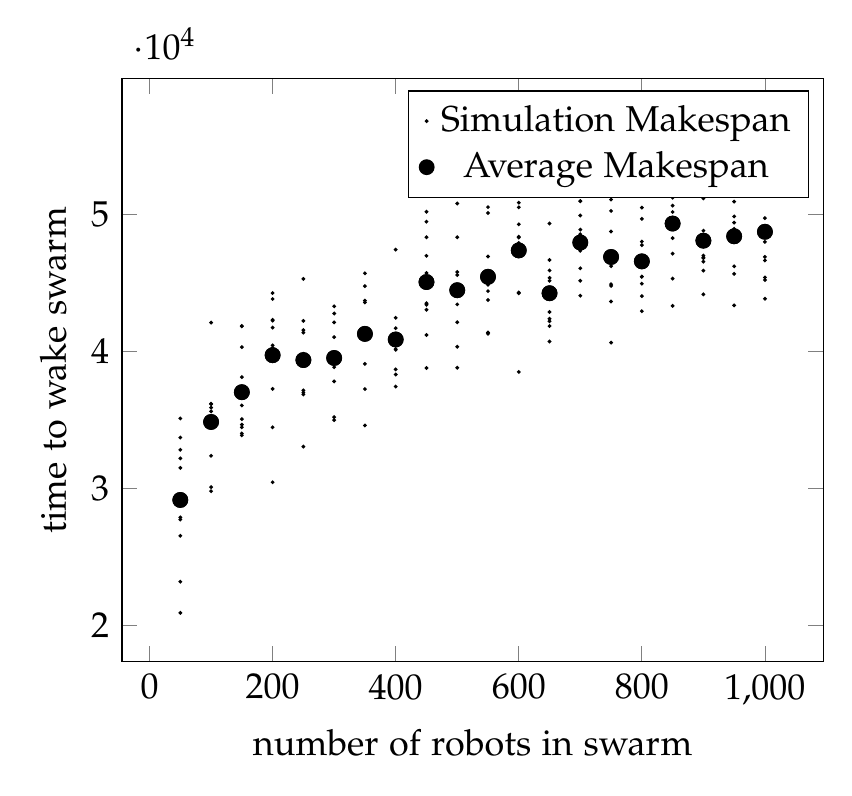
\begin{tikzpicture}[scale=1.3]
\begin{axis}[
scatter/classes={
    a={draw=black, mark=*, mark size=0.3}, b={draw=black}},
xlabel={number of robots in swarm}, ylabel={time to wake swarm}]
\addplot[scatter,only marks, scatter src=explicit symbolic]
table[meta=label] {
x y label
50 27733 a
50 32198 a
50 26546 a
50 31504 a
50 35113 a
50 33717 a
50 23201 a
50 20926 a
50 32824 a
50 27893 a
50 29165 b
100 42109 a
100 35626 a
100 29803 a
100 35107 a
100 36188 a
100 36155 a
100 30104 a
100 32390 a
100 35900 a
100 35189 a
100 34857 b
150 34469 a
150 35068 a
150 41839 a
150 38133 a
150 33886 a
150 40319 a
150 34016 a
150 34664 a
150 36060 a
150 41861 a
150 37031 b
200 37269 a
200 41746 a
200 40440 a
200 40258 a
200 42312 a
200 30456 a
200 34469 a
200 43830 a
200 44267 a
200 42254 a
200 39730 b
250 37162 a
250 45296 a
250 41563 a
250 33061 a
250 39346 a
250 36867 a
250 41381 a
250 37008 a
250 39835 a
250 42234 a
250 39375 b
300 42773 a
300 34992 a
300 35213 a
300 38853 a
300 43300 a
300 39469 a
300 37817 a
300 39684 a
300 42127 a
300 41048 a
300 39527 b
350 34601 a
350 45706 a
350 41453 a
350 39094 a
350 43581 a
350 41465 a
350 41208 a
350 43711 a
350 44771 a
350 37260 a
350 41285 b
400 37440 a
400 38318 a
400 47433 a
400 41703 a
400 40123 a
400 41226 a
400 40178 a
400 38694 a
400 41187 a
400 42457 a
400 40875 b
450 48337 a
450 43521 a
450 45726 a
450 38791 a
450 49474 a
450 46980 a
450 43043 a
450 43412 a
450 41202 a
450 50202 a
450 45068 b
500 38814 a
500 48338 a
500 40343 a
500 45796 a
500 44836 a
500 42132 a
500 50801 a
500 45580 a
500 43438 a
500 44659 a
500 44473 b
550 45374 a
550 45827 a
550 46937 a
550 44871 a
550 50537 a
550 50114 a
550 43763 a
550 41294 a
550 44407 a
550 41381 a
550 45450 b
600 50521 a
600 38510 a
600 47920 a
600 44249 a
600 50862 a
600 44304 a
600 49281 a
600 48383 a
600 51441 a
600 48316 a
600 47378 b
650 42886 a
650 40731 a
650 49341 a
650 42204 a
650 41855 a
650 45156 a
650 45372 a
650 42388 a
650 46680 a
650 45917 a
650 44253 b
700 48556 a
700 47353 a
700 46071 a
700 45162 a
700 48894 a
700 47538 a
700 49923 a
700 50979 a
700 50970 a
700 44074 a
700 47952 b
750 51679 a
750 51091 a
750 46228 a
750 43648 a
750 46989 a
750 44787 a
750 44912 a
750 48757 a
750 40648 a
750 50258 a
750 46899 b
800 47758 a
800 44041 a
800 42940 a
800 44947 a
800 48025 a
800 45453 a
800 49681 a
800 50498 a
800 45471 a
800 46969 a
800 46578 b
850 53247 a
850 49260 a
850 54749 a
850 50646 a
850 43334 a
850 47138 a
850 48276 a
850 45323 a
850 50180 a
850 51223 a
850 49337 b
900 46866 a
900 48813 a
900 47004 a
900 45903 a
900 51173 a
900 46817 a
900 46554 a
900 44172 a
900 51886 a
900 51682 a
900 48087 b
950 48323 a
950 48293 a
950 45667 a
950 49406 a
950 49856 a
950 46218 a
950 43364 a
950 48955 a
950 50937 a
950 53063 a
950 48408 b
1000 45402 a
1000 46904 a
1000 43851 a
1000 52368 a
1000 46645 a
1000 52859 a
1000 45216 a
1000 48003 a
1000 56372 a
1000 49734 a
1000 48735 b
};
\addplot[scatter,only marks, scatter src=explicit symbolic]
table[meta=label] {
x y label
50 29165 b
100 34857 b
150 37031 b
200 39730 b
250 39375 b
300 39527 b
350 41285 b
400 40875 b
450 45068 b
500 44473 b
550 45450 b
600 47378 b
650 44253 b
700 47952 b
750 46899 b
800 46578 b
850 49337 b
900 48087 b
950 48408 b
1000 48735 b
};

\legend{Simulation Makespan, Average Makespan}

\end{axis}
\end{tikzpicture}
\end{figure}
\begin{multicols}{2}
\section{Experiment}
\subsection{Experiment Setup}
The experiment is based on a Python 2.7.9 simulation of swarms of varying sizes where the robots are running an implementation of the Nearest Neighbor Algorithm. The simulations were performed on a 64-bit PC running Linux OS.
\paragraph{Dataset.} The simulations are run with 210 different geometric datasets consisting of increasing numbers of robots randomly placed on a $10000 \times 10000$ unit two dimensional Euclidean plane. The release time of each robot is a random number between 0 and 5000 time units. The source robot is the first robot placed on the plane.
\paragraph{Parameters.} Robots were given a movement speed of 1 unit of geometric space per 1 unit of time.
\paragraph{Performance Measure} The performance of the algorithm on the datasets is based solely on the makespan. 

\subsection{Experiment Results}
In our plot the horizontal axis corresponds to the number of robots in the swarm. The vertical axis corresponds with the makespan of the simulation. Small dots are the results of individual runs of the simulation and the large dots are the average of all runs for the given swarm size.

\section{Future Work}
It would be interesting to explore other heuristics for the OTDFTP as well as test other dataset types such as grid swarm arrangement using the Nearest Neighbor algorithm.
%----------------------------------------------------------------------------------------
%	REFERENCE LIST
%----------------------------------------------------------------------------------------

\bibliography{bibliography}{}
\bibliographystyle{plain}

%----------------------------------------------------------------------------------------

\end{multicols}

\end{document}
\grid
